%!TEX root = ../../csuthesis_main.tex

\chapter{类脑视觉模型理论基础}

\section{人类视觉系统启发机制}

\subsection{视觉皮层的层级结构与功能分区}

人类视觉系统是感知系统中最复杂的部分之一,承担了大脑约30\%以上的皮层资源。其结构具有高度分化的层级性与区域功能分区,形成了自下而上与自顶向下并行交互的处理机制。以腹侧通路(ventral visual pathway)为代表的信息流动路径,从初级视觉皮层(V1)逐层向上延伸至中间层(V2、V4)与高级层(IT),在每一层均完成不同层级的特征加工与抽象表示\cite{ kanwisher2010functional}。

\begin{figure}[hbt]
	\centering
	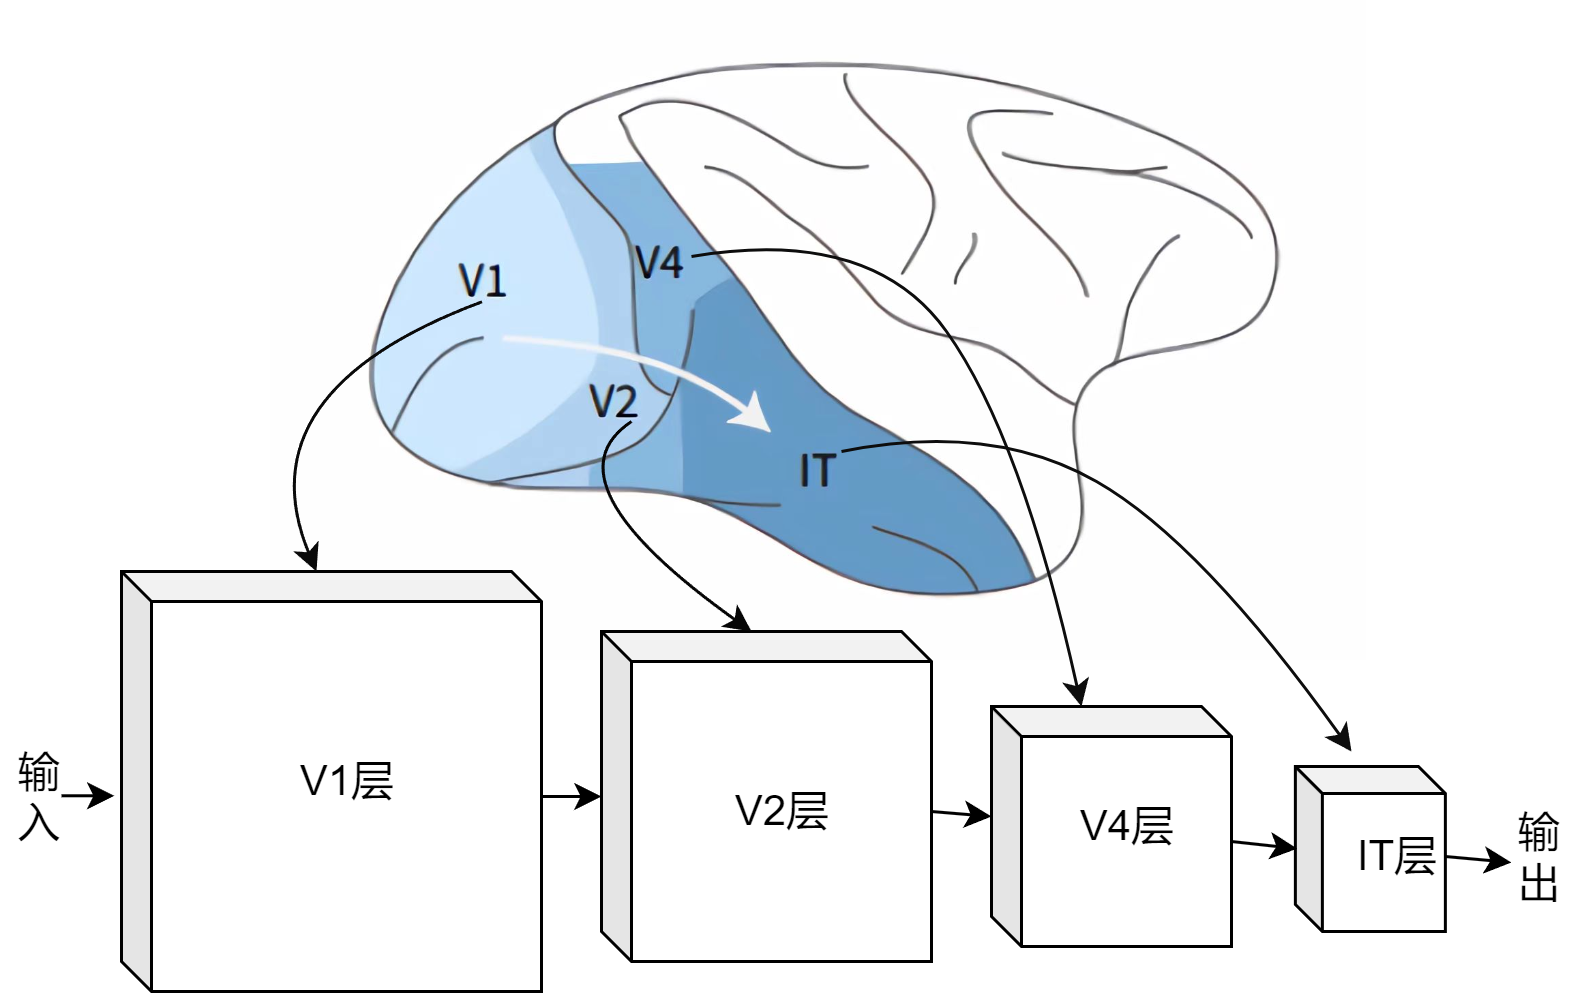
\includegraphics[width=0.5\linewidth]{brain.jpg}
	\caption{人类视觉皮层信息流路径示意图}
	\label{f.naoquyu}
\end{figure}

V1区域被称为“初级视觉皮层”,主要处理图像中的低级视觉特征,如边缘、方向、空间频率和亮度对比等。其神经元具有较小的感受野,排列有序,形成“列结构”以支持对特定方向的偏好响应。这些特征构成了后续感知加工的基础。V2区域作为V1的上一级处理层,结合多个V1神经元的输出,开始在边缘连接、曲率、角度整合等更复杂结构层面提取图像信息。
V4区通常被认为是颜色与形状知觉的关键节点,其神经元对复杂几何结构与颜色组合有强烈反应,是从“几何特征”到“语义物体”之间的桥梁区域。在大多数视觉认知模型中,V4所建构的中层表示具有显著的判别性。

IT(Inferotemporal Cortex,颞下皮层)则是腹侧通路中处理最高阶语义信息的区域,神经元对复杂物体类别具有极高的选择性和不变性,甚至可以对面孔、动物等类别展现出特定偏好,是完成目标识别与恒常性表征的终点区域。

这套层级结构不仅沿空间方向递进,每一层还存在纵向的功能模块分区。例如在IT区内,存在“面孔选择性区域(face-selective patches)”,专门处理人脸类视觉信息。这种功能分区的特点也启发了深度网络中使用模块化设计与结构对齐策略。

值得一提的是,这些视觉皮层区域并不是孤立运行的,它们通过大量前馈(feedforward)与反馈(feedback)通路构成动态交互体系,不同区域之间的连接支持了多尺度特征融合与时间维度上的认知更新,为类脑模型的递归结构设计提供了重要依据\cite{yamins2016using}。

以CORnet模型为例,它的网络结构就是参考这种自底向上的层级构造:通过将V1、V2、V4和IT模块分别模拟生物视觉系统的不同处理阶段,模型能够在保持较少参数量的同时,模拟视觉特征由低到高的提取路径。这种结构的设计不仅提升了神经对应性,也为后续通过Brain-Score等类脑评估工具进行模块对齐提供了技术基础。

\subsection{反馈调节与时间动态特性}

在人类的视觉系统中,信息的处理并不是仅仅沿着自下而上的前馈路径逐级传递,越来越多的研究表明,自顶向下的反馈连接在感知过程中扮演着不可或缺的调节角色。反馈机制不仅有助于整合高层的语义信息、强化有意义的特征,还参与了注意力控制、错误预测修正和不确定性分辨等认知过程,是构成大脑动态信息处理系统的关键环节。

视觉皮层中的反馈连接广泛存在于V1至V2、V4及IT等多个区域之间,特别是在目标识别、遮挡补全、模糊图像感知等复杂情境下,反馈回路被激活以引导底层区域重构或调整特征表征。例如,当输入图像包含模糊或不完整信息时,高层区域如IT可将先验经验通过反馈信号传递回V1或V2,引导低级区域生成可能的轮廓或结构,从而提高识别的鲁棒性\cite{wyatte2014early}。此外,反馈路径还被发现与注意力调控密切相关,大脑可通过该机制优先激活与当前任务目标相关的感受野区域,实现特征选择性增强\cite{bastos2012canonical}。

除了结构性反馈外,视觉系统还具有显著的时间动态特性,即感知过程不仅是瞬时处理,而且是在数十至数百毫秒的时间窗口内逐步建立稳定表征。这种动态更新不仅反映在神经元活动持续时间上,还包括反应延迟、阶段性加工与反应强度调节等因素。研究发现,目标识别并非在一次前馈过程中完成,而是经过多个循环、信息在区域间往返传播,形成一种接近“递归建模”的处理模式\cite{kar2019evidence}。

受此启发,近年来类脑视觉模型在结构设计上也逐步引入时间维度的建模方式。如CORnet-R模型加入局部递归单元,模拟区域内的短时反馈;CORnet-S模型更进一步,引入跨层级递归结构和时间步展开,使得模型可在多个时间状态下动态整合信息,从而更贴近真实神经系统的加工流程\cite{kubilius2019brain}。这种时间展开机制不仅提升了模型对遮挡、旋转和噪声图像的识别能力,也增强了其在神经预测任务中的表现。

通过对反馈调节与时间动态的结构建模,不仅可以提升模型的判别性能,更为类脑模型引入了“过程性认知”的基础,有望拓展其在多任务感知与长期记忆建构方面的研究潜力。


\subsection{注意力机制在神经计算中的作用}

在人类视觉系统中,注意力机制是一种高效的信息调节手段,能够根据当前任务、环境或内在动机,对大量感知输入进行筛选、放大与抑制,从而优化认知资源的分配。其本质就是一种选择性加工机制,使大脑在资源有限的条件下,优先处理对行为目标最相关的信息。这种机制广泛存在于从早期视觉皮层V1到高级皮层IT的多个层级,并在视觉识别、空间定位、目标追踪等任务中发挥关键作用。

从神经生理的角度看,注意力调节表现为特定神经元群体的兴奋增强与非目标区域神经元响应的抑制。当个体集中注意于某一刺激或区域时,相应皮层区域内神经元的放电频率明显提高,而非关注区域的活动水平则下降,形成“兴奋—抑制”的对比调节模式。这种神经活动的空间聚焦与通道加权现象,为后续人工网络中注意力模块的设计提供了重要启发\cite{carrasco2011visual}。

在神经计算模型中,注意力机制不仅能够提升模型对关键信息的响应灵敏度,还能够增强模型在复杂场景下的鲁棒性与泛化能力。近年来,越来越多的深度学习结构开始主动引入生物启发式的注意力模块,如通道注意力(Channel Attention)、空间注意力(Spatial Attention)以及时序注意力(Temporal Attention)等。其中,Squeeze-and-Excitation(SE)模块通过学习每一特征通道的重要性来调节通道权重,模拟了神经元对不同刺激类型的响应偏好\cite{hu2018squeeze};而CBAM模块进一步结合空间选择性处理,更接近大脑中多层次调控的注意机制\cite{woo2018cbam}。

有研究还表明,注意力机制还与大脑的预测编码能力密切相关。在面对不确定或模糊刺激时,大脑通过基于经验的预测来“填补”感知信息的空缺,而注意机制则辅助定位最需修正的信息区域。这一过程被认为与前额叶皮层和视觉皮层之间的反馈回路密切相关,是实现“自上而下”调节的重要手段\cite{bastos2012canonical}。

国内学者们也在注意力机制的类脑建模方面展开了研究。如刘建伟等人提出,多模态注意力机制在模拟人脑对图像、语言、声音等多源信息的联合选择方面具有显著优势,并对其神经基础进行了系统梳理,为后续视觉-语义耦合类脑系统设计提供了理论参考\cite{刘建伟2020多模态深度学习综述}。

综合来看,注意力机制不仅是人脑感知系统中不可或缺的组成部分,也是当前类脑视觉模型提升生物合理性与任务适应能力的重要设计元素。其生理基础的不断深入理解,正在推动人工智能模型从“结构还原”向“功能对齐”迈进。


\section{CORnet模型架构解析}

\subsection{CORnet-Z与CORnet-S模型结构比较}

CORnet(Core Object Recognition network)系列的类脑视觉模型模型是由MIT的Kubilius等人提出的,目的是为了构建结构与功能均尽量贴近灵长类视觉系统的深度神经网络。该模型家族的命名灵感来源于“大脑核心视觉识别能力”(core object recognition),通过模块化设计与时间动态建模,尝试在轻量化架构中重现人类在静态图像识别中的部分认知机制\cite{kubilius2019brain}。

CORnet-Z模型是这个模型系列中最基础的版本,它的架构包括四个连续的模块:V1、V2、V4和IT,分别对应着生物视觉通路中的四个皮层区域。每个模块都由一个卷积层、ReLU激活函数和最大池化操作组成,用于模拟特定层级的感受野增大和特征抽象过程。该结构通过模仿大脑的视觉功能区域划分,在卷积神经网络的基本框架上实现了初步的神经解剖对齐。模型的输出通过全局平均池化和全连接层进入分类器,形成标准的图像识别流程。由于不含递归、跳跃或多尺度融合结构,CORnet-Z模型的整体架构十分简洁、计算效率高,便于调试与神经表征可视化,常用于类脑模型的对照实验与基线评估。

相比之下,CORnet-S模型在Z版本的基础上进一步引入了时间步机制和局部递归连接,以更接近灵长类大脑在时间维度上的信息处理特性。其核心模块CORblock-S在每一层内部设置了多个“时间步”,同一输入在不同时刻被重复处理,实现了内部状态随时间演化的能力。这一设计灵感源于神经科学中关于大脑“再入处理(reentry)”机制的发现,即高层皮层区域会通过反馈路径影响低层区域的激活状态,从而实现自上而下的调节与预测修正\cite{kar2019evidence}。CORnet-S模型的递归结构允许高阶语义信息通过时间传播机制调整前级特征的响应,有助于增强网络在遮挡、模糊与目标干扰等复杂视觉情境下的稳定性。

实验结果表明,在Brain-Score平台提供的神经预测任务中,CORnet-S模型在V4与IT层均取得了比CORnet-Z更高的一致性得分,显示出更优的类脑表征能力\cite{kubilius2019brain}。该结果说明引入递归与时间机制不仅提升了模型对复杂输入的表达能力,也在一定程度上模拟了真实大脑中上下行回路的信息整合过程。

在计算资源消耗方面,两者存在明显差异。CORnet-Z由于结构浅、无时间展开,其参数总量小、推理速度快,适合在边缘设备上部署,也便于开展结构模块的插拔实验。CORnet-S尽管结构更接近生物视觉皮层,但时间维度的递归计算显著增加了训练成本和模型复杂度。两者在性能、类脑相似性与可操作性之间各有权衡,可根据研究目标灵活选用。

总的来看,CORnet-Z适合用作结构对比与模块测试的类脑模型基线,而CORnet-S则可用于探讨反馈调节、动态表征等更接近生物神经系统的机制,在类脑建模研究中形成了互为补充的关系。两者在性能与类脑性之间各有侧重。

\begin{table}[htbp]
	\centering
	\caption{CORnet系列模型结构对比}
	\begin{tabular}{l|c|c|c}
		\hline
		& CORnet-Z & CORnet-R & CORnet-S \\
		\hline
		V1 &
		\begin{tabular}[c]{@{}c@{}}conv 7$\times$7/2 \\ maxpool 3$\times$3/2\end{tabular} &
		\begin{tabular}[c]{@{}c@{}}conv 7$\times$7/4 \\ conv 3$\times$3\end{tabular} &
		\begin{tabular}[c]{@{}c@{}}conv 7$\times$7/2 \\ maxpool 3$\times$3/2 \\ conv 3$\times$3\end{tabular} \\
		\hline
		V2 &
		\begin{tabular}[c]{@{}c@{}}conv 3$\times$3 \\ maxpool 3$\times$3/2\end{tabular} &
		\begin{tabular}[c]{@{}c@{}}conv 3$\times$3/2 \\ conv 3$\times$3\end{tabular} &
		\begin{tabular}[c]{@{}c@{}}conv 1$\times$1 \\ conv 1$\times$1\\ conv 3$\times$3/2 \\ conv 1$\times$1\end{tabular} \\
		\hline
		V4 &
		\begin{tabular}[c]{@{}c@{}}conv 3$\times$3/2 \\ maxpool 3$\times$3/2\end{tabular} &
		\begin{tabular}[c]{@{}c@{}}conv 3$\times$3/2 \\ conv 3$\times$3\end{tabular} &
		\begin{tabular}[c]{@{}c@{}}conv 1$\times$1 \\ conv 1$\times$1\\ conv 3$\times$3/2 \\ conv 1$\times$1\end{tabular} \\
		\hline
		IT &
		\begin{tabular}[c]{@{}c@{}}conv 3$\times$3/2 \\ maxpool 3$\times$3/2\end{tabular} &
		\begin{tabular}[c]{@{}c@{}}conv 3$\times$3/2 \\ conv 3$\times$3\end{tabular} &
		\begin{tabular}[c]{@{}c@{}}conv 1$\times$1 \\ conv 1$\times$1\\ conv 3$\times$3/2 \\ conv 1$\times$1\end{tabular} \\
		\hline
	\end{tabular}
	\label{tab:cornet_z_r_s_compare}
\end{table}

\subsection{CORnet模型的类脑设计理念与评价依据}

CORnet系列模型设计的一个核心理念就是实现“结构可对应、功能可解释”。这一理念的目的在于使人工神经网络不仅在表现上接近人类,还能在结构与功能机制上具备明确的生物学对应关系。模型中的每个模块均明确对照大脑视觉皮层中的特定区域,例如V1、V2、V4和IT,其内部结构通过卷积层模拟不同脑区的感受野响应和特征加工过程,层级处理顺序也严格遵循腹侧视觉通路的进阶逻辑:从初级边缘与方向提取,到中间层的形状组合,再到高级的对象语义识别\cite{dicarlo2012does}。这种“区域映射式”的模块化命名与结构设定,使得每一个模型子结构都可与神经科学中的真实皮层区域进行比较,为后续的神经一致性分析、可解释性评估以及可视化操作提供了良好基础。

在评估维度上,CORnet系列被广泛用于Brain-Score等平台的标准测试中。Brain-Score平台整合了包括非人灵长类电生理记录、人类行为响应和图像识别任务在内的多维度数据,提供了一套从神经响应到认知行为的统一模型评估体系。该平台通过将模型中间层输出与真实神经元反应进行相关性比较,例如在V4评估中,研究者会提取模型V4模块的激活响应,并使用线性回归或RDM方法预测猴子V4区的神经放电率。得分越高说明模型对该脑区的模拟能力越强,大脑相似度就越高。CORnet-Z作为结构简洁的前馈模型,在V4与IT层的得分中表现尚可,但受限于其缺乏动态建模机制,整体神经一致性得分与实际大脑仍存在一定差距。

CORnet-S则在此基础上通过时间递归机制增强了模型对再入处理与上下文调节的表达能力,使其在IT层的神经一致性表现优于Z版本,接近于部分标准CNN模型在行为任务中的表现(如ResNet-50)。该模型因结构透明、逻辑简洁且评估结果稳定,被视为当前类脑建模中的结构与功能结合较好的一类代表性模型。

此外,CORnet系列模型结构本身具有高度的可扩展性,便于研究者在其基础上进行结构优化与功能增强。例如,可以在IT模块中插入注意力机制(如SE或CBAM)、递归循环单元或生物启发式感受野建模模块,也可在V1模块中引入Gabor滤波、VOneBlock等神经建模方法以模拟低级神经响应特性。这种“开放式模块嵌入”能力使得CORnet成为构建定制化类脑视觉系统的理想平台。

同时,模型官方代码已完全开源,并基于PyTorch深度学习框架实现,支持GPU加速训练、灵活的模块重构与中间层可视化。随着Brain-Score社区的持续更新,CORnet模型已成为类脑视觉领域中最常用的起始基线之一,也被越来越多研究用于类脑系统对比分析、结构变体评估与神经层级对齐研究。

\section{类脑相似性评估基准}

\subsection{Brain-Score指标体系}

衡量人工神经网络是否具备类脑特性,不能只是依赖传统准确率指标,而应从模型的神经响应模式、层级功能和行为输出等多维度进行分析。近年来,随着脑神经记录技术与计算模型的结合,建立起一系列神经一致性评估工具,其中以Brain-Score平台为代表,逐步形成较为系统的类脑模型评价标准。

Brain-Score是由MIT、Harvard等研究机构联合提出的一套类脑评估框架,旨在系统评估人工神经网络在模拟生物视觉系统方面的能力。该体系融合了神经科学实验数据与人工智能模型的行为输出,通过与灵长类动物的神经反应和人类行为表现进行量化对比,从而为“类脑性”提供一个客观、可复现的标准化评价指标\cite{schrimpf2018brain}。

Brain-Score的设计逻辑建立在“大脑不同区域对视觉信息的层级加工”这一神经生理学基础之上。平台提供了包括猴子V4和IT皮层的神经电生理记录数据,以及人类在目标识别任务中的行为数据,构成三类主要评估维度:神经预测得分(Neural Predictivity)、行为一致性(Behavioral Similarity)与层级表征对齐度(Layer Correspondence)。

其中,神经预测得分指标是评估重点。该任务要求模型在输入相同刺激图像后,其中间层输出通过线性映射能够准确预测真实神经元的响应。预测精度采用皮尔逊相关系数(Pearson Correlation Coefficient)进行计算:

\begin{equation}
	r = 
	\frac{
		\sum_{i=1}^{n}(y_i - \bar{y})(\hat{y}_i - \bar{\hat{y}})
	}{
		\sqrt{\sum_{i=1}^{n}(y_i - \bar{y})^2} \cdot \sqrt{\sum_{i=1}^{n}(\hat{y}_i - \bar{\hat{y}})^2}
	}
	\label{eq:pearson}
\end{equation}
其中,$y_i$表示真实神经响应值,$\hat{y}_i$为模型预测值,$n$为图像样本数。对每个神经元单独计算相关系数后,Brain-Score 以所有神经元得分的平均值作为最终神经预测得分:

\begin{equation}
	\text{Brain-Score}_{\text{layer}} = \frac{1}{m} \sum_{j=1}^{m} r_j
	\label{eq:brain_score}
\end{equation}
其中$m$为目标脑区中的神经元数量,$r_j$为第$j$个神经元的Pearson得分。

在模型比较中,该得分范围为$[0, 1]$,得分越高表示模型越能模拟目标脑区的神经响应模式。目前,Brain-Score已成为国际上衡量类脑视觉模型标准化水平的主流指标体系,广泛应用于CNN、Transformer、类脑建模等多个领域的模型评估研究中,其数据集与评估标准仍在持续更新扩展,逐步推动类脑人工智能系统的跨学科发展。

\subsection{神经数据对齐机制}

在类脑视觉模型的神经预测评估中,一个关键步骤是实现模型中间层输出与神经记录数据之间的表征对齐。这一过程的核心在于构建一种能够将人工神经网络的特征向量映射到生物神经元响应空间的函数关系,从而衡量二者之间的相似程度。当前Brain-Score所采用的标准方法是偏最小二乘回归(Partial Least Squares,PLS),其本质是一种在高维特征下实现稳健线性映射的降维拟合方法,尤其适用于样本数量远小于特征维度的场景\cite{hair2019use}。

Brain-Score假设模型特征$X \in \mathbb{R}^{n \times d}$与神经响应矩阵$Y \in \mathbb{R}^{n \times m}$存在以下线性映射关系:

\begin{equation}
	Y = XW + \varepsilon
	\label{eq:linear_model}
\end{equation}
其中$W$为待学习的投影矩阵,$\varepsilon$为高斯噪声项。训练过程中,系统对$W$进行拟合,并通过交叉验证控制过拟合。最终,使用训练好的映射将测试集上的模型特征映射为神经预测值$\hat{Y}$,再计算其与真实神经响应$Y$的相关性。

由于大多数深度神经网络中间层的维度远高于神经元采样数量(如模型特征维度为数千而神经元数量不足数百),直接进行线性映射容易导致过拟合或数值不稳定。因此,在实际操作中,常先对模型特征进行主成分分析(PCA)降维处理,保留90\%以上的累计贡献率。这样可在压缩特征维度的同时保持信息完整性,确保PLS映射过程的稳定性。

\begin{figure}[hbt]
	\centering
	
\includegraphics[width=0.8\linewidth]{数据处理流程图.png}
	\caption{数据处理流程图}
	\label{f.sjcllct}
\end{figure}

该机制不仅能够对模型结构是否“类脑”给出量化评估,还具有较强的解释力。研究者可以进一步分析哪些特征维度在预测神经元活动中起主导作用,进而调整模型结构以靠近生物神经编码特性。这种“神经对齐机制”已经成为当前类脑建模研究中最具可操作性和比较性的核心方法之一。

目前,Brain-Score所使用的PLS回归方法在静态图像上的一致性评价取得了良好效果,但其仍存在一定局限性。一是评估所使用的数据是以静止、中心注视图像为主,难以覆盖自然视觉场景中的动态变化、遮挡、光照扰动等因素。二是该方法假设模型表征与神经活动之间存在线性关系,尚未能处理更为复杂的非线性响应或时间动态特性。此外,当前框架中对主动注意力调节、行为选择偏好等高阶认知机制的类脑建模仍较为薄弱。

尽管如此,Brain-Score的神经对齐机制仍为现阶段类脑模型评估提供了统一标准和高度可复现的操作流程,在模型结构调优、类脑反馈机制设计与认知对齐分析等方面均发挥着重要参考价值。

